
\begin{figure}[!h]
    \centering
    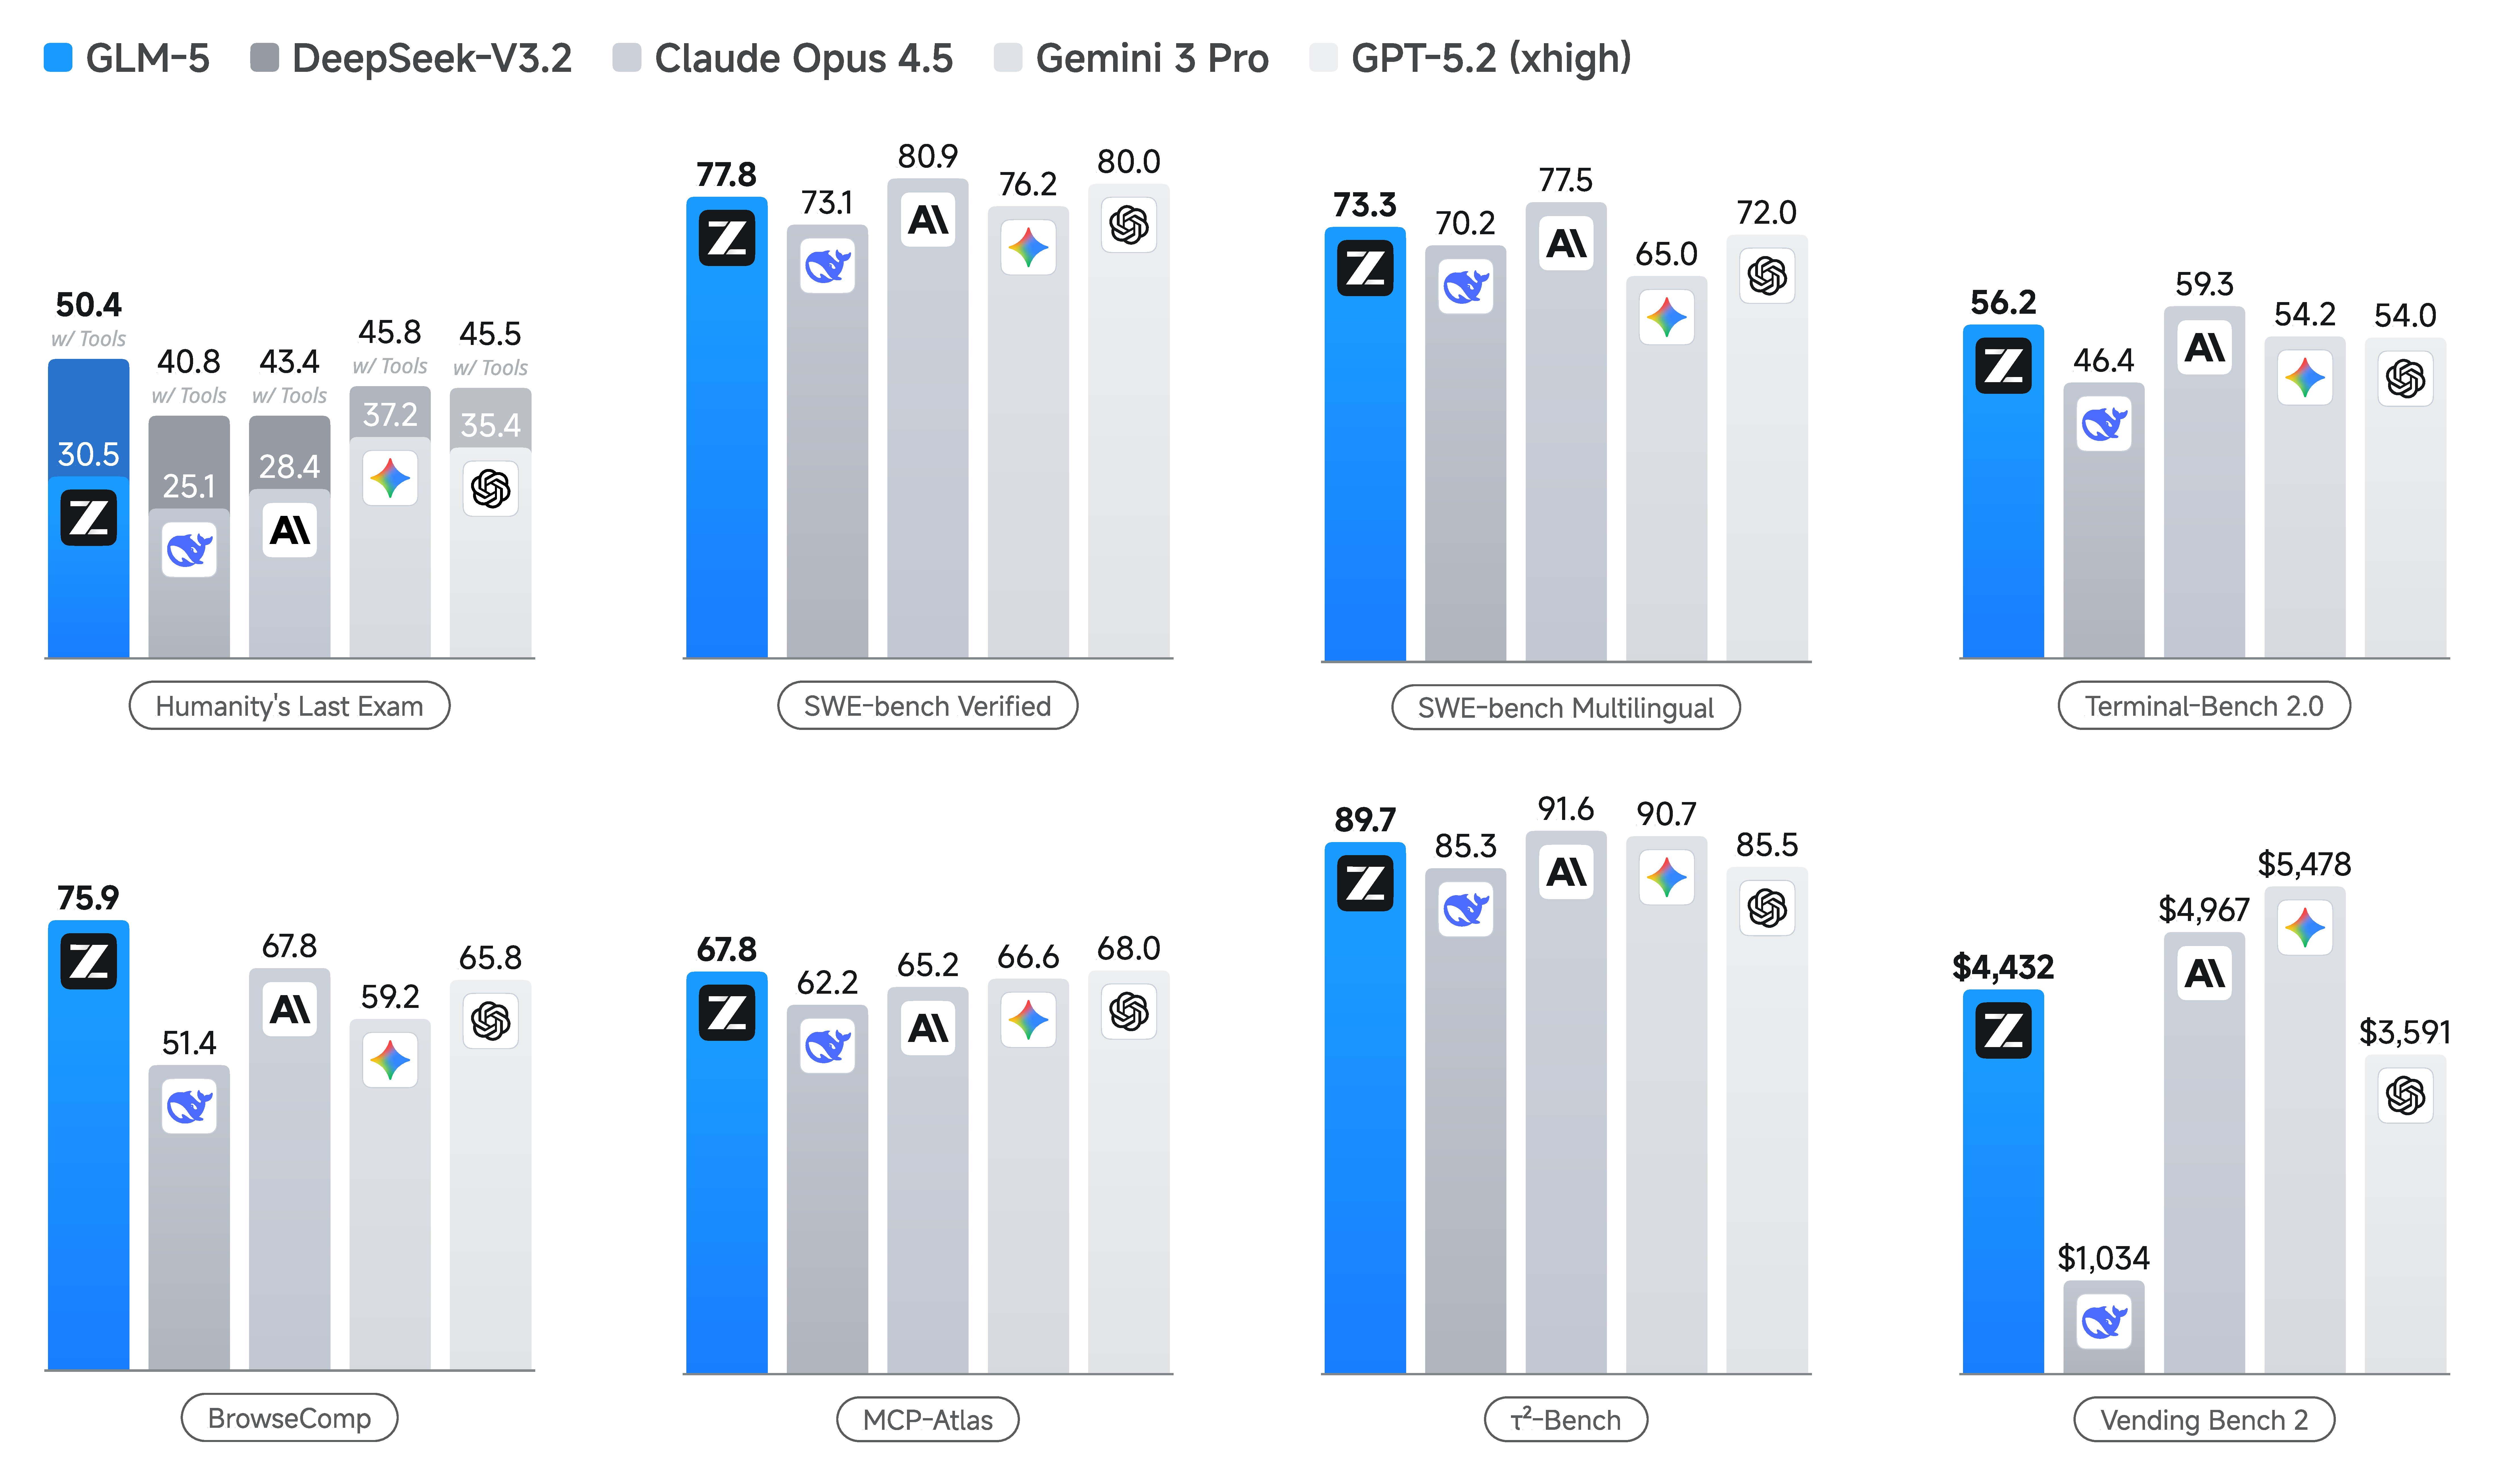
\includegraphics[width=\linewidth]{figures/arc_clean.pdf}
    \caption{GLM-5、DeepSeek-V3.2、Claude Opus 4.5、Gemini 3 Pro 和 GPT-5.2（xhigh）在 8 个智能体、推理与编码基准上的结果：Humanity's Last Exam、SWE-bench Verified、SWE-bench Multilingual、Terminal-Bench 2.0、BrowseComp、MCP-Atlas、$\tau^2$-Bench、Vending Bench~2。}
    \label{fig:arc}
\end{figure}


\section{引言}

追求通用人工智能（AGI）不仅需要扩大模型参数规模，也需要从根本上重思智能效率与自主改进架构。随着 GLM-4.5 的发布，我们证明了将 Agentic、Reasoning 和 Coding（ARC）能力统一到单一 Model-of-Experts（MoE）架构中，可以在多类基准上取得最先进结果。然而，随着大语言模型（LLM）从被动知识存储器转向主动问题求解器，计算成本与真实世界适应性（尤其在复杂软件工程中）这两大挑战，已成为主要瓶颈。

我们提出 GLM-5——新一代旗舰模型，旨在突破这些障碍。GLM-5 在性能与效率上都实现了范式跃迁：在 ArtificialAnalysis.ai、LMArena Text、LMArena Code 等主要公开榜单上达到最先进水平。更重要的是，GLM-5 重新定义了真实世界编码标准，展现出处理复杂端到端软件开发任务的前所未有能力，远超 SWE-bench 等传统静态基准所覆盖的范围。

\paragraph{结果。} 图~\ref{fig:arc} 展示了 GLM-5、GLM-4.7、Claude Opus 4.5、Gemini 3 Pro 与 GPT-5.2（xhigh）在 8 个智能体、推理与编码基准上的表现：Humanity's Last Exam~\cite{phan2025humanity}、SWE-bench Verified~\cite{jimenez2023swe}、SWE-bench Multilingual~\cite{yang2025swemulti}、Terminal-Bench 2.0~\cite{tbench_2025}、BrowseComp~\cite{wei2025browsecomp}、MCP-Atlas~\cite{bandi2026mcp}、$\tau^2$-Bench~\cite{yao2024tau,barres2025tau2}、Vending Bench 2~\cite{backlund2025vending}。平均来看，GLM-5 相比上一版本 GLM-4.7 提升约 20\%，与 Claude Opus 4.5、GPT-5.2（xhigh）大体相当，并优于 Gemini 3 Pro。

GLM-5 在 Intelligence Index v4.0 上达到 50 分，成为新的开源权重榜首（见图~\ref{fig:aa}）；相较 GLM-4.7 的 42 分提升了 8 分，提升主要来自智能体性能与知识/幻觉控制。这也是开源权重模型首次在 Artificial Analysis Intelligence Index v4.0 上达到 50 分。

\begin{figure}[t]
    \centering
    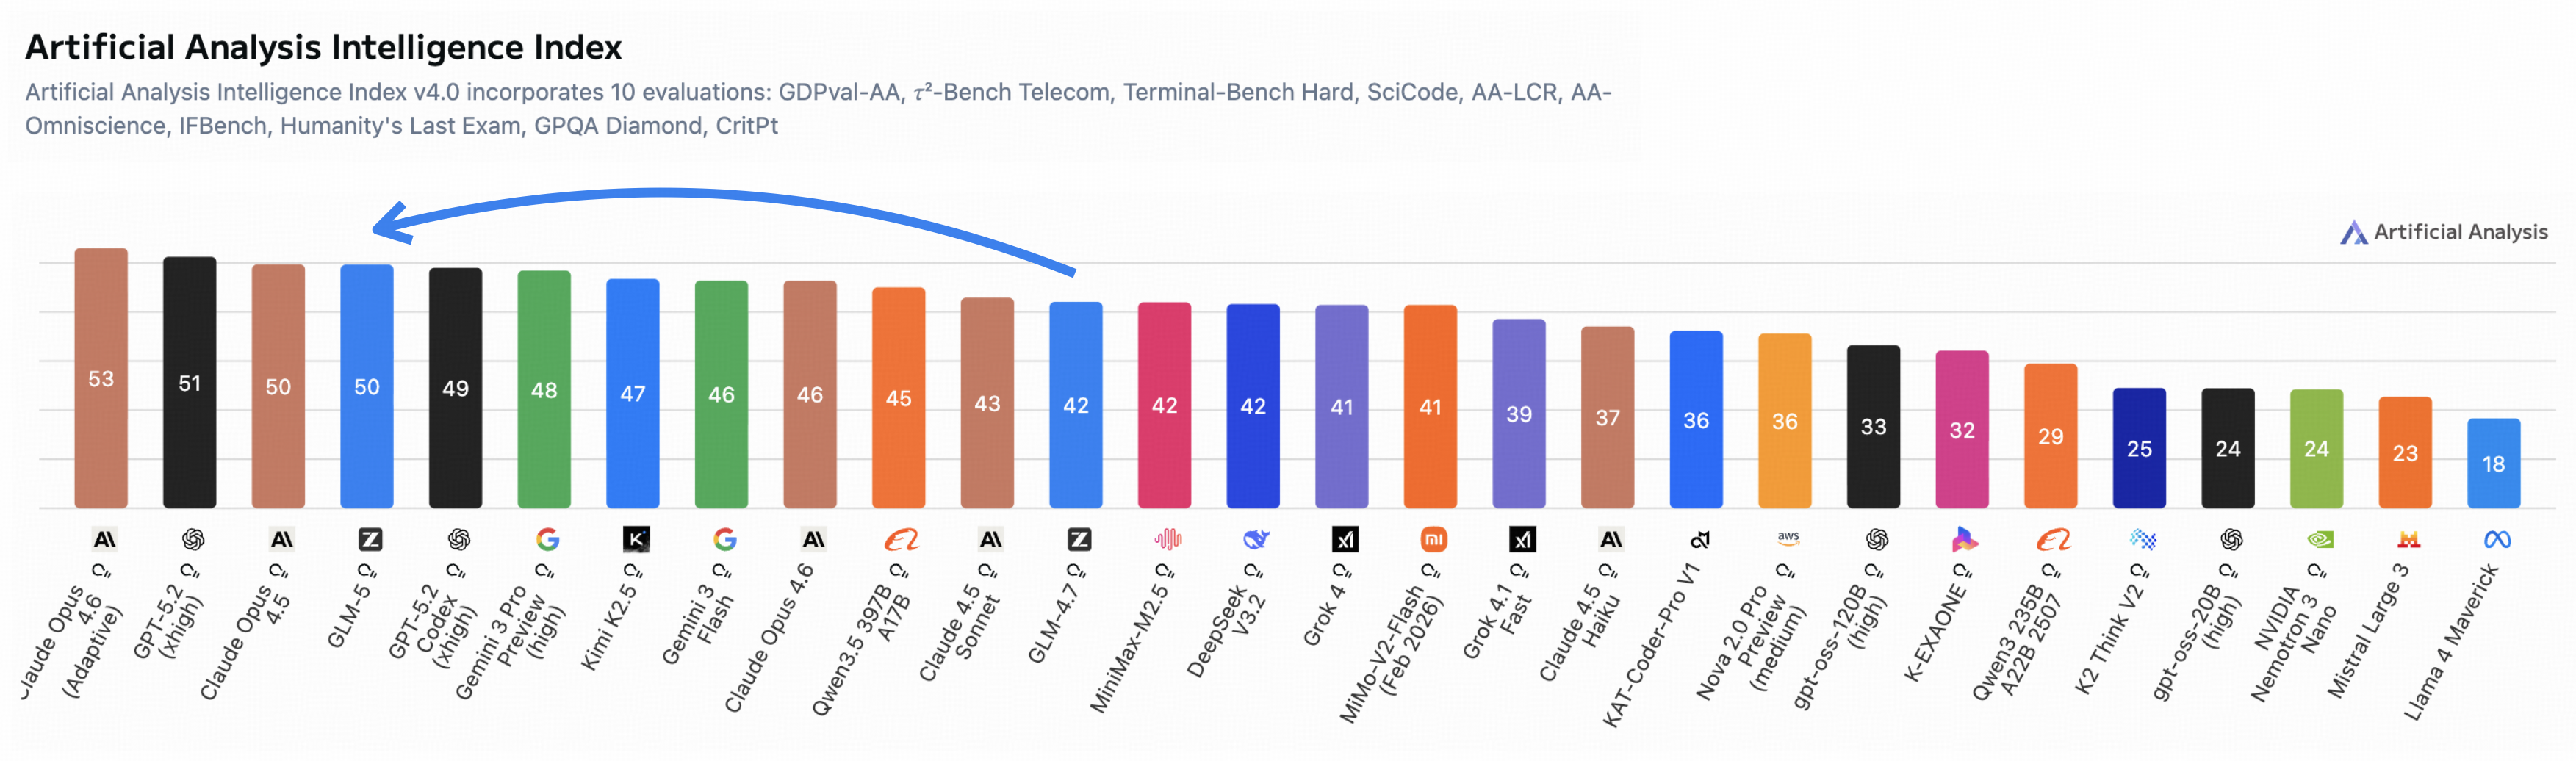
\includegraphics[width=1\linewidth]{figures/aa.PNG}
    \caption{Artificial Analysis Intelligence Index v4.0 包含 10 项评测：GDPval-AA、$\tau^2$-Bench Telecom、Terminal-Bench Hard、SciCode、AA-LCR、AA-Omniscience、IFBench、Humanity's Last Exam、GPQA Diamond、CritPt。}
    \label{fig:aa}
\end{figure}

\begin{figure}[t]
    \centering
    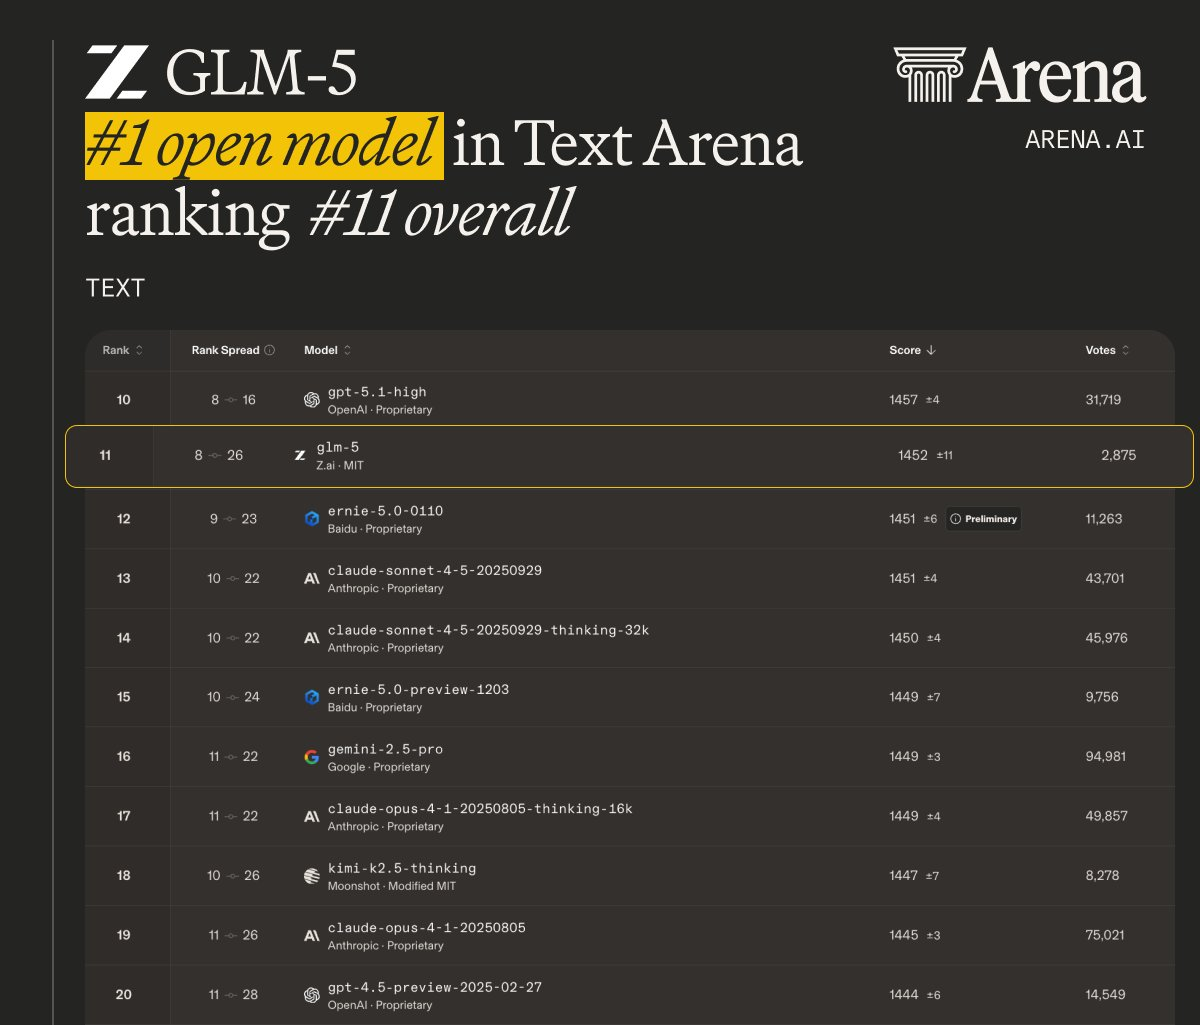
\includegraphics[width=0.48\linewidth]{figures/text-arena.jpeg} \;\;\;
    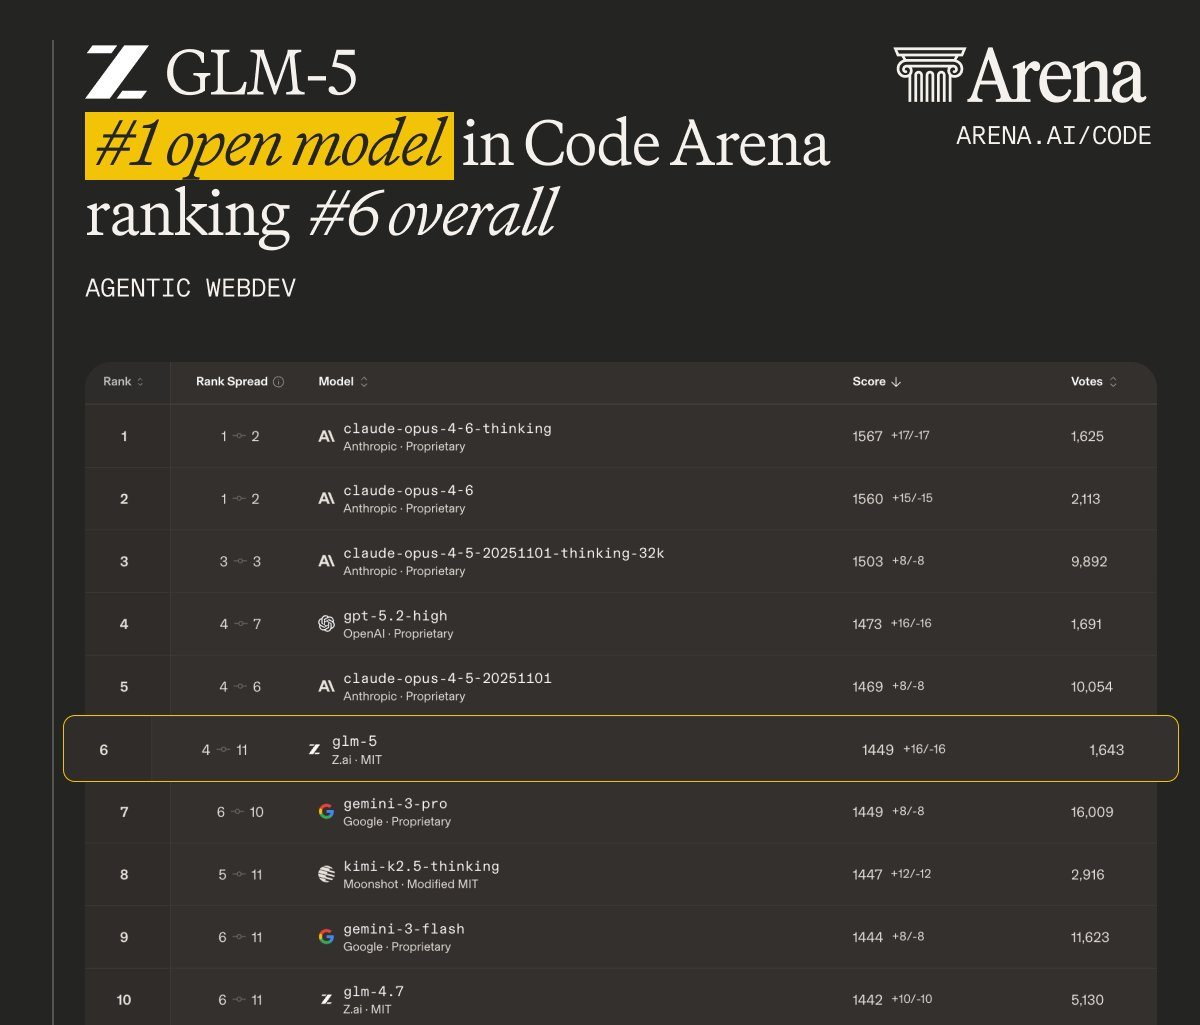
\includegraphics[width=0.48\linewidth]{figures/code-arena.jpeg}
    \caption{在 LMArena 上，GLM-5 在 Text Arena 与 Code Arena 均为 \#1 开源模型。}
    \label{fig:arena}
\end{figure}

\begin{figure}[t]
    \centering
    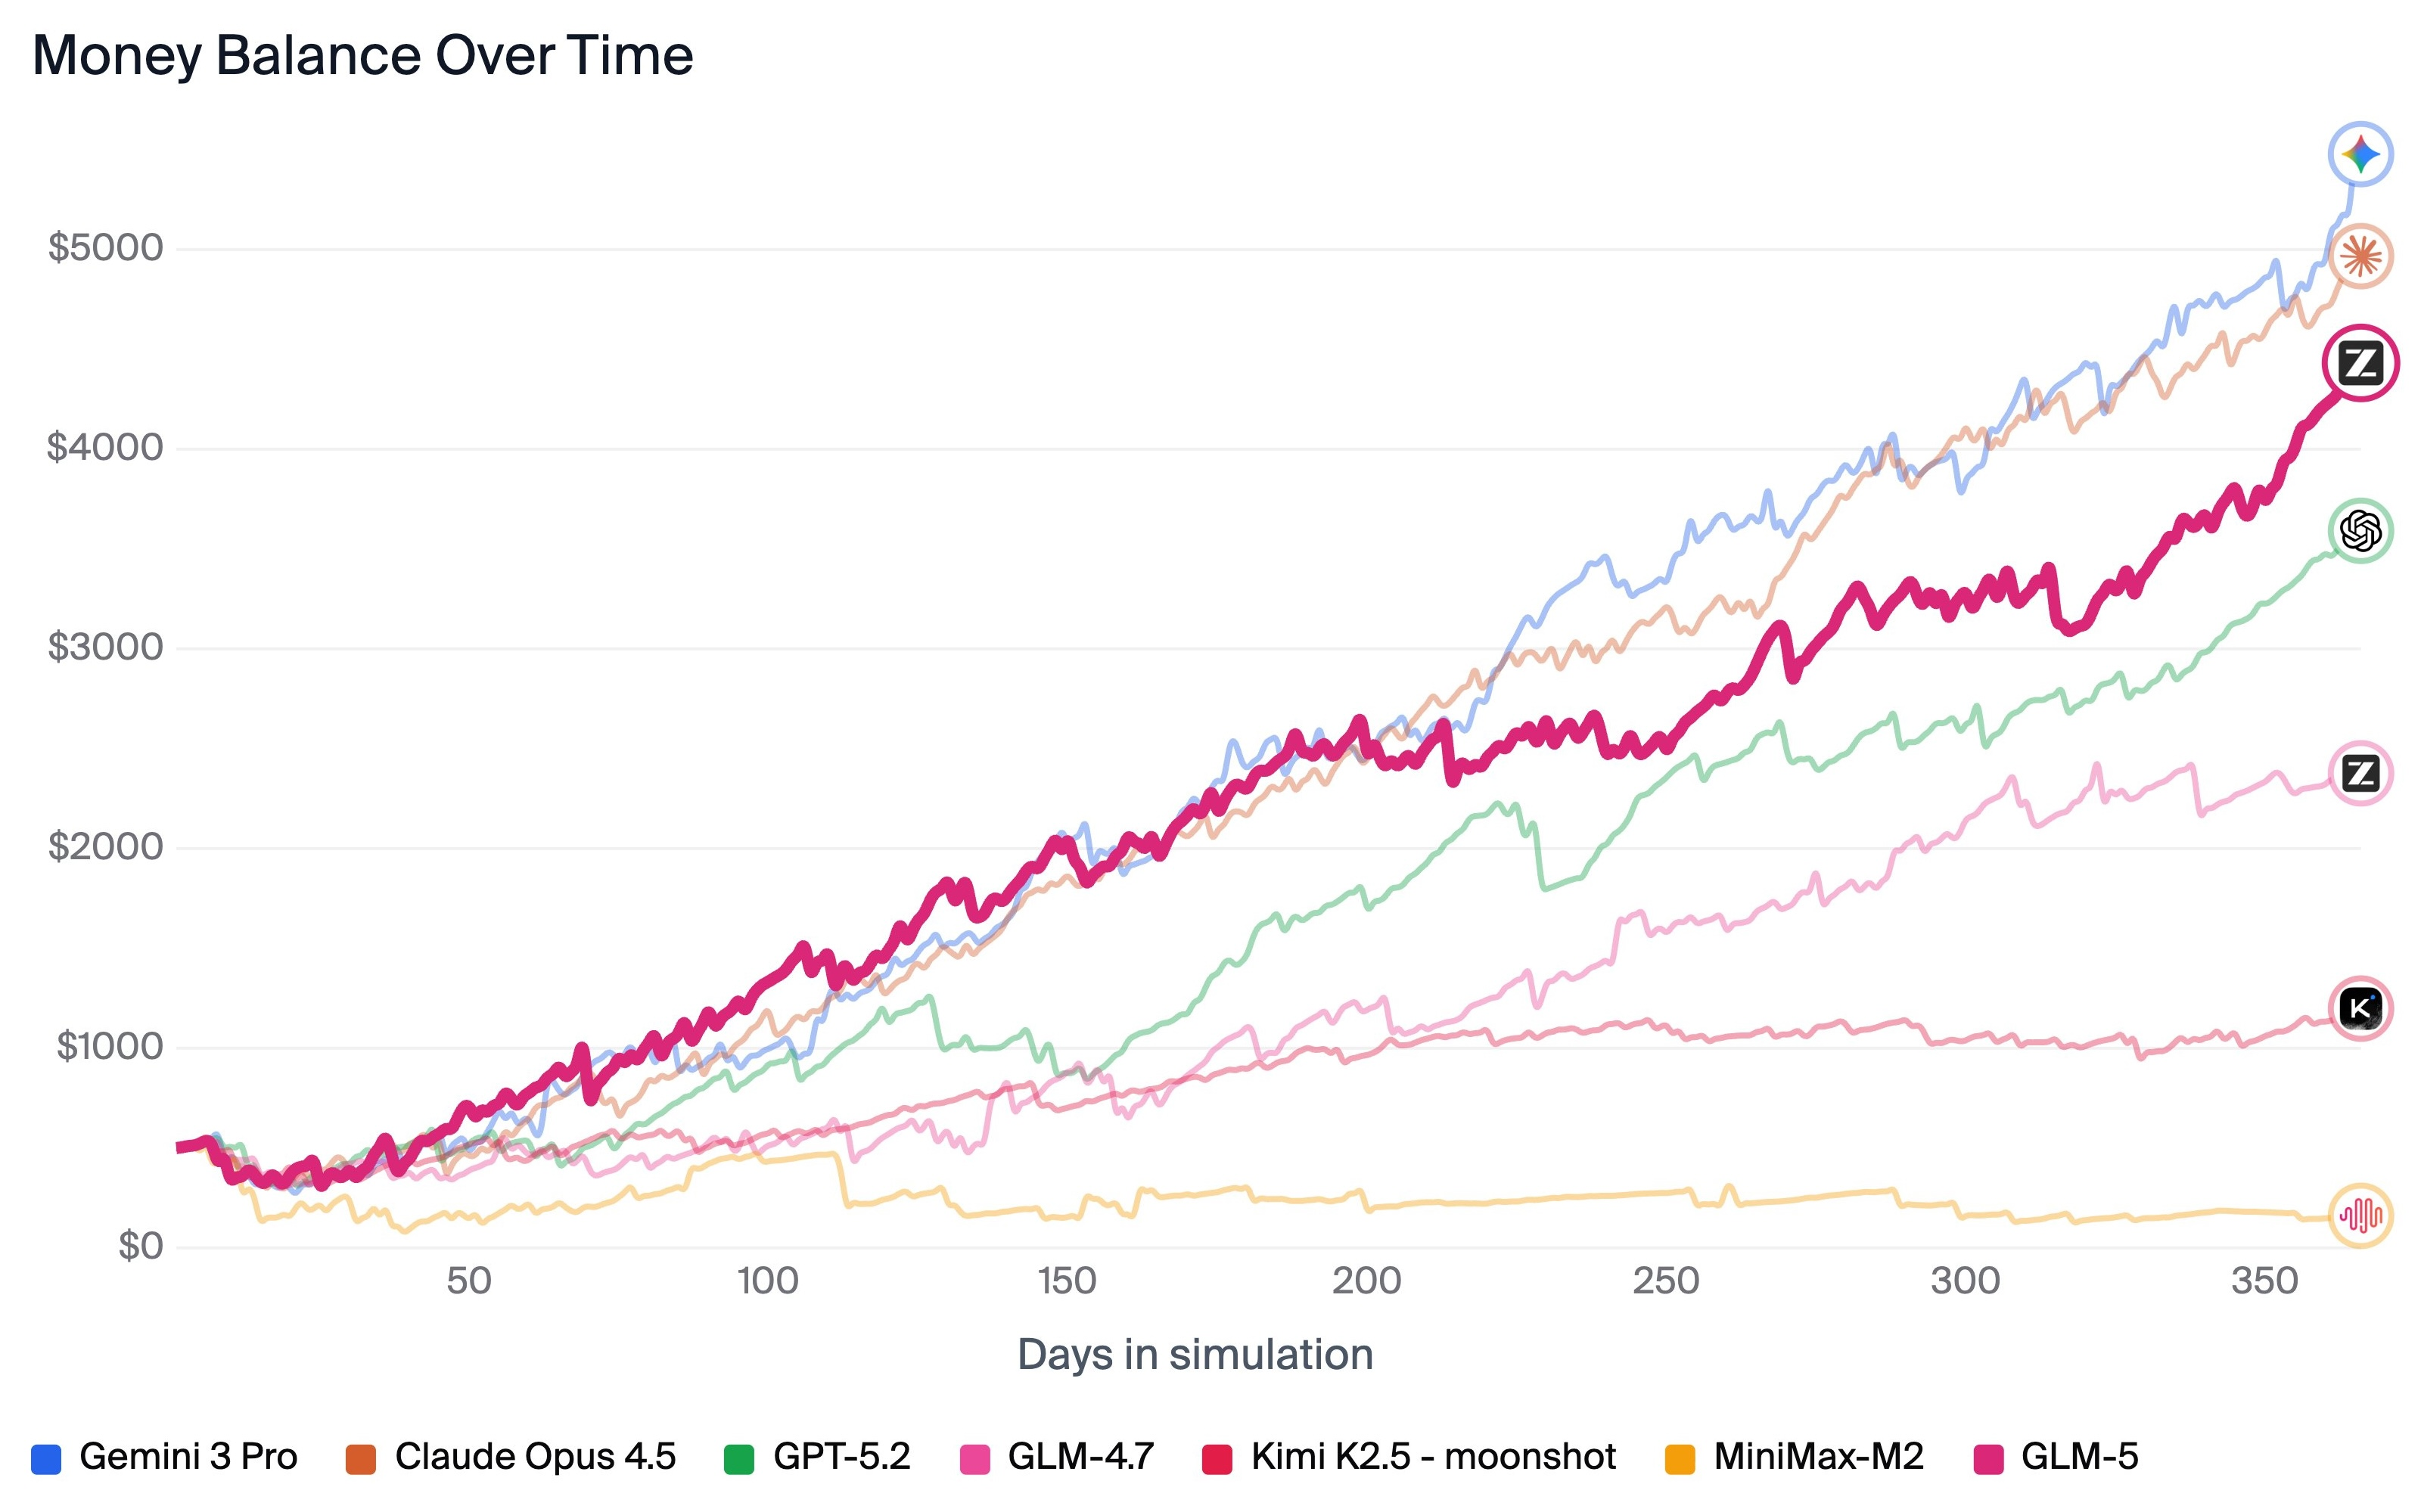
\includegraphics[width=0.50\linewidth]{figures/vending-bench.jpeg} \;\;
    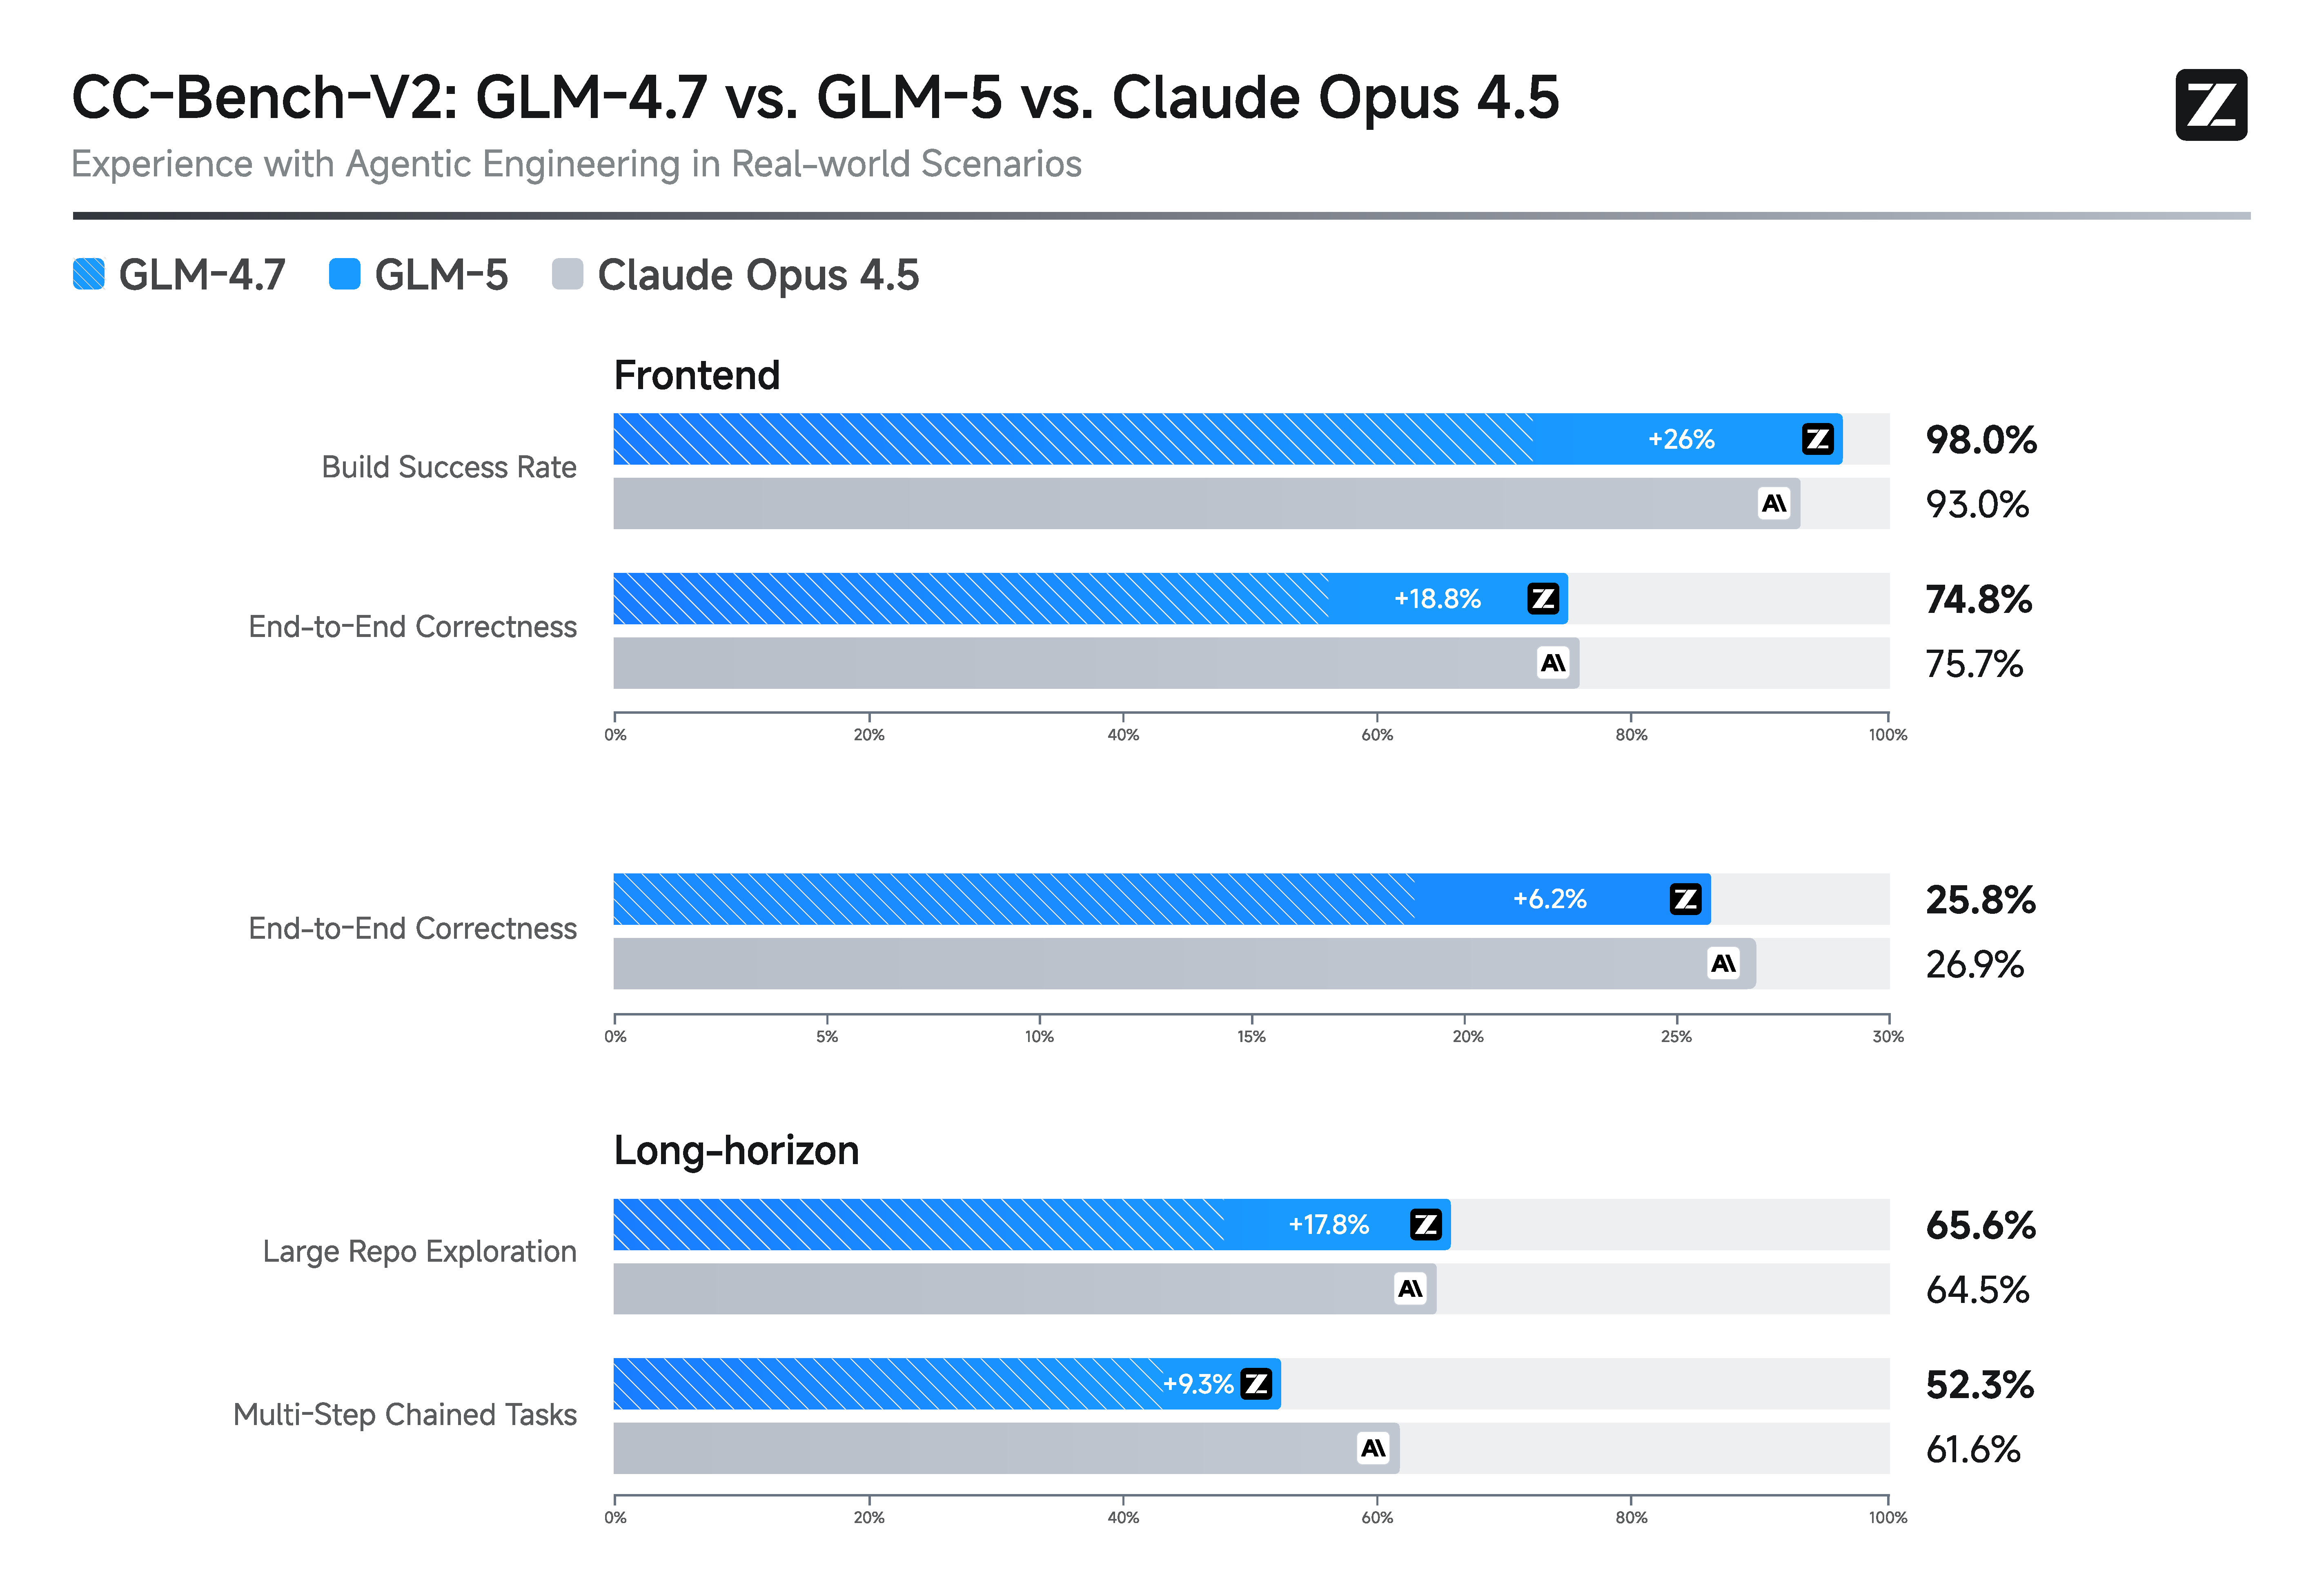
\includegraphics[width=0.47\linewidth]{figures/cc-bench-v2.pdf}
    \caption{若干长时程任务结果。左：Vending-Bench 2；右：CC-Bench-V2。}
    \label{fig:vendingcc}
\end{figure}

LMArena 由 UC Berkeley 发起，是一个透明共享的平台，通过人类评判在数百万真实任务上评估并比较前沿 AI 能力，任务包括写作、编码、推理、设计、搜索与创作。大规模人类交互产生了真实世界效用信号，这使其区别于其他静态基准。
图~\ref{fig:arena} 显示，GLM-5 再次成为 Text Arena 与 Code Arena 的 \#1 开源模型，总体
与 Claude-Opus-4.5 和 Gemini-3-pro 处于同一水平。


智能体的长期一致性正变得越来越重要。编码智能体如今可以自主编程数小时，AI 模型可完成任务的长度与广度也将持续提升。我们使用 Vending-Bench 2 与 CC-Bench-V2 两个基准评估 GLM-5 完成长时程任务的能力。
Vending-Bench 2 用于衡量 AI 模型在长期经营业务中的表现。模型需要在模拟自动售货机场景中运营一年，并按期末银行账户余额评分。
图~\ref{fig:vendingcc}（左）显示，GLM-5 在所有开源模型中排名 \#1，期末账户余额达到 \$4,432。其表现接近 Claude Opus 4.5，体现出较强的长期规划与资源管理能力。
图~\ref{fig:vendingcc}（右）进一步展示了我们内部评测套件 CC-Bench-V2 的结果。GLM-5 在前端、后端和长时程任务上均显著优于 GLM-4.7，并缩小了与 Claude Opus 4.5 的差距。


\begin{figure}[t]
    \centering
    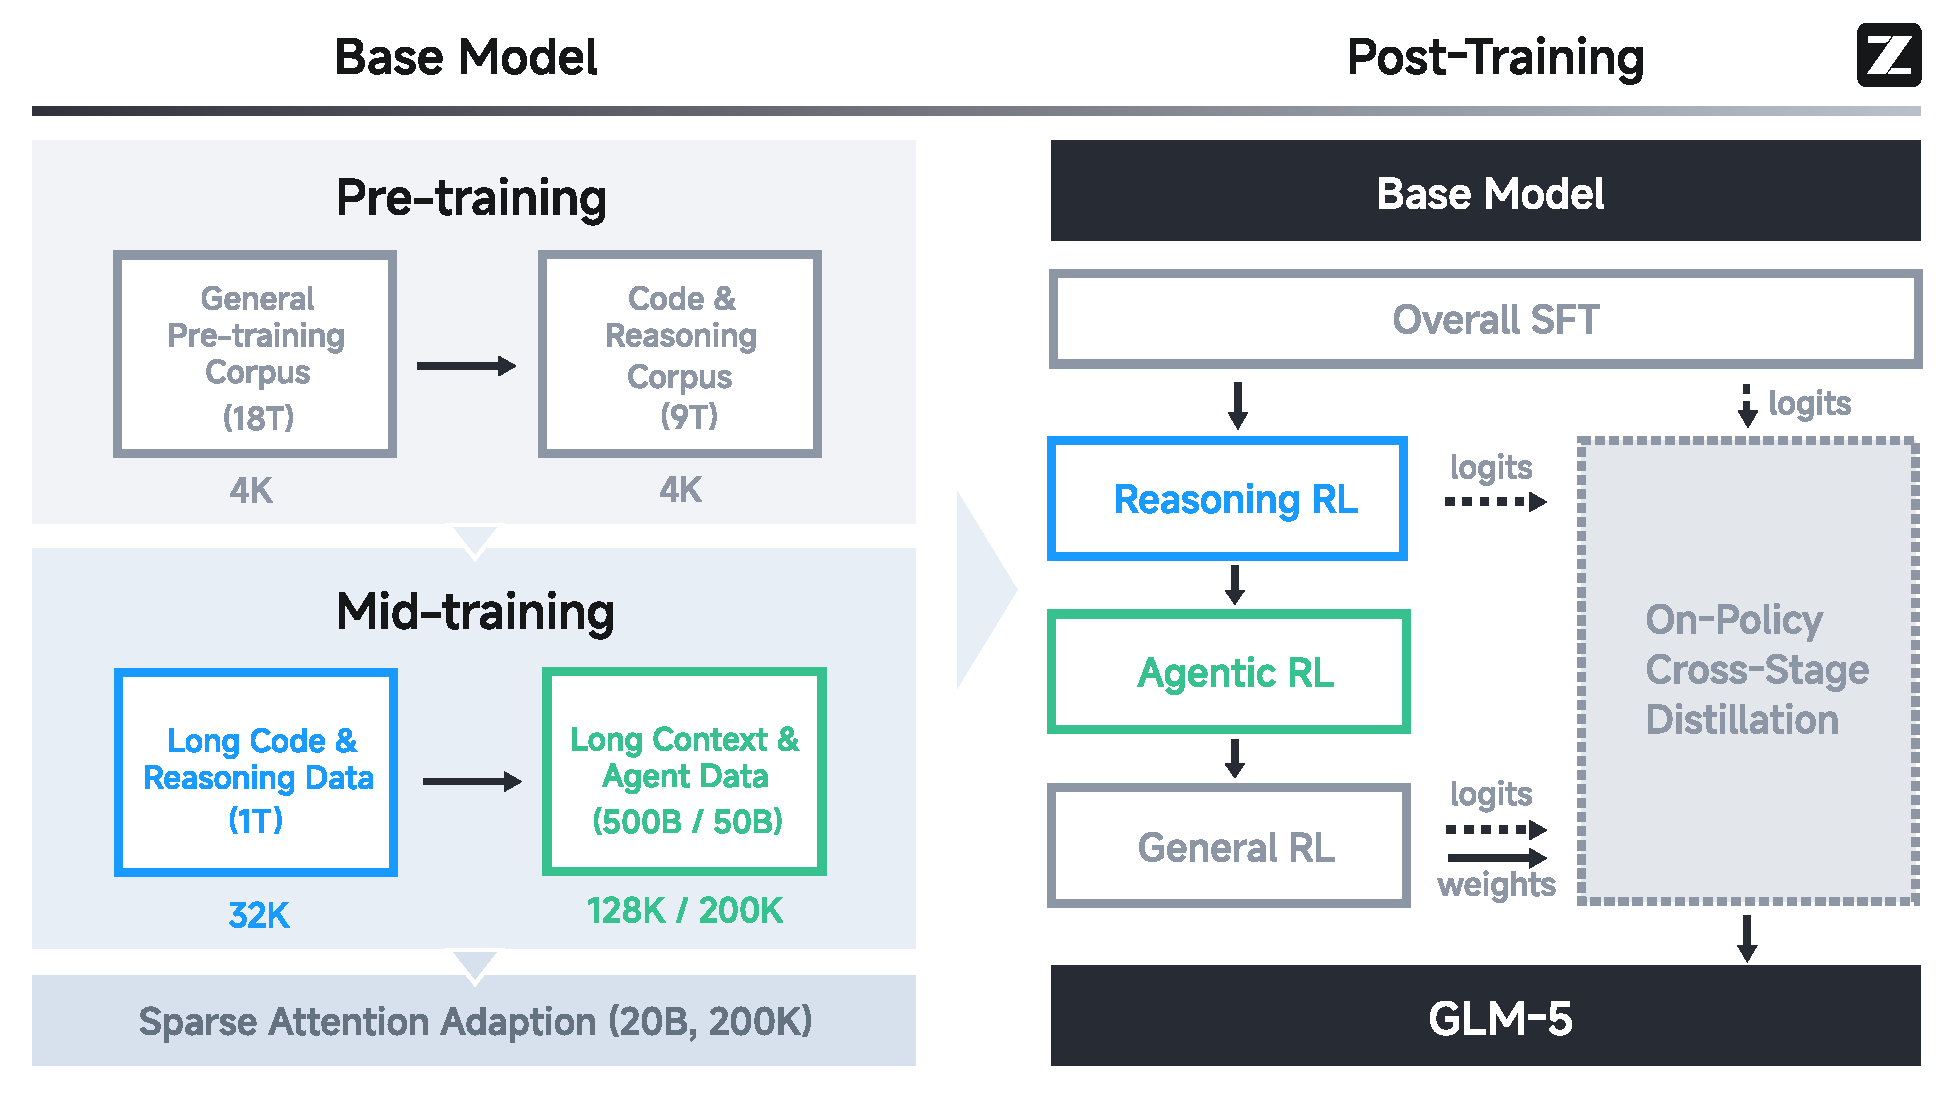
\includegraphics[width=1\linewidth]{figures/overall_pipeline.pdf}
    \caption{GLM-5 的整体训练流程。}
    \label{fig:overall_pipeline}
\end{figure}

\paragraph{方法。} 图~\ref{fig:overall_pipeline} 展示了 GLM-5 的整体训练流程。
我们的基座模型训练从一个大规模 27 万亿 token 语料库开始，并在早期优先关注代码与推理。随后我们采用独立的中期训练阶段，将上下文长度从 4K 渐进扩展到 200K，重点使用长上下文智能体数据，以确保复杂工作流中的稳定性。
在后训练阶段，我们超越了标准 SFT。我们实现了顺序化强化学习流水线——先进行推理 RL，再进行智能体 RL，最后进行通用 RL。关键在于，我们在全过程中使用 On-Policy Cross-Stage Distillation 来防止灾难性遗忘，确保模型在成为强大通才的同时保留锋利的推理能力。
总之，GLM-5 的性能跃升主要由以下技术贡献驱动：

首先，我们采用 DSA（DeepSeek Sparse Attention）~\cite{deepseekai2025deepseekv32pushingfrontieropen}，这是一项新型架构创新，可显著降低训练与推理成本。尽管 GLM-4.5 已通过标准 MoE 架构提升效率，DSA 仍能依据 token 重要性动态分配注意力资源，在不牺牲长上下文理解和推理深度的前提下大幅降低计算开销。借助 DSA，我们将模型参数规模提升至 744B，并将训练 token 预算扩展至约 28.5T。

其次，我们构建了新的异步强化学习基础设施。基于 ``slime'' 框架以及在 GLM-4.5 中初始化的解耦 rollout 引擎，新基础设施进一步将生成与训练解耦，以最大化 GPU 利用率。该系统支持对智能体轨迹进行大规模探索，避免了过去限制迭代速度的同步瓶颈，显著提升了 RL 后训练流水线效率。

第三，我们提出了新型异步 Agent RL 算法，以提升自主决策质量。在 GLM-4.5 中，我们采用迭代式自蒸馏与结果监督来训练智能体。对于 GLM-5，我们开发了异步算法，使模型能够持续地从多样化、长时程交互中学习。这些算法专门针对动态环境中的规划与自我纠错能力进行优化，直接促成了我们在真实世界编码场景中的领先表现。

最后，另一个技术贡献在于：GLM-5 从第一天起就对中国 GPU 生态进行全栈适配。我们已在包括华为昇腾、摩尔线程、海光、寒武纪、昆仑芯、沐曦、燧原在内的 7 个主流国产芯片平台上，完成了从底层 kernel 到上层推理框架的深度优化。

凭借这些进展，GLM-5 不只是一个更强大的模型，更是下一代 AI 智能体更高效、更实用的基础。我们将 GLM-5 开源给社区，以进一步推动高效、智能体化通用智能的前沿发展。
